\subsection{Häufige Funktionsgraphen}
    \centerline{
        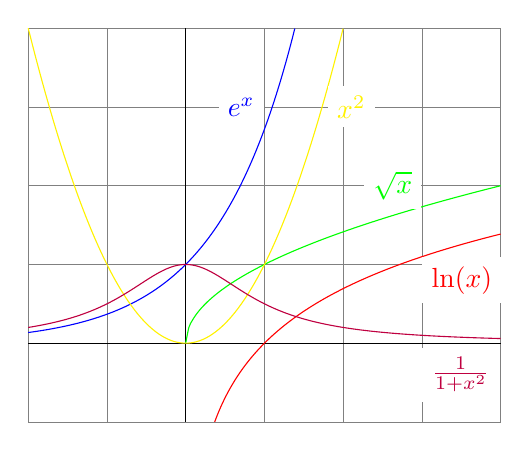
\begin{tikzpicture}
            \draw [help lines] (-2,-1) grid [step=1] (4,4);
            \draw (-2,0) -- (4,0);
            \draw (0,-1) -- (0,4);
            \draw [color = red] plot [smooth, samples = 100, domain = 0.368:4] (\x, {ln(\x)});
                \draw (3, 0.8) node[right, red, fill=white] {$\ln(x)$};
            \draw [color = blue] plot [smooth, samples = 100, domain = -2:1.386] (\x, {e^\x});
                \draw (1,3) node[left, blue, fill=white] {$e^x$};
            \draw [color = green] plot [smooth, samples = 100, domain = 0:4] (\x, {sqrt(\x)});
                \draw (3,2) node[left, green, fill=white] {$\sqrt{x}$};
            \draw [color = yellow] plot [smooth, samples = 100, domain = -2:2] (\x, {(\x)^2});
                \draw (1.8, 3) node[right, yellow, fill=white] {$x^2$};
            \draw [color = purple] plot [smooth, samples = 100, domain = -2:4] (\x, {1/(1+(\x)^2)});
                \draw (3,-0.4
                ) node[right, purple, fill=white] {$\frac{1}{1+x^2}$};
        \end{tikzpicture}
    }